\section{Introduction}
Entanglement-based quantum key distribution (QKD) relies on a steady source of photon pairs. The first step in establishing a key in such a scheme is the assignment of photodetection events to entangled photon pairs \cite{ho2009clock}. Due to their strong temporal correlation (down to a few 100 fs) in typical pair sources, this assignment can be done via temporal coincidence identification. However, complexity from Doppler shift rates at different angles of elevation can cause this cross correlation to be spread out over thousands of time bins. This note details two methods for correcting Doppler effects in satellite-to-ground coincidence matching. 

\subsection{Time stamping a satellite SPDC source}

We consider a setup where a spontaneous parametric down conversion (SPDC) source on a satellite is time stamped by two individual time stamp cards with a relative clock drift of 165$\mu$s/s (Fig \ref{fig:spdc_source}).\\ 

\begin{figure}[ht!]
	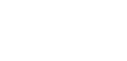
\includegraphics[width=\linewidth]{assets/spdc_source}
	\caption{Idlers and 1\% of signal photons are time-stamped on the satellite. The rest of the signal photons are transmitted to ground.}
	\label{fig:spdc_source}
\end{figure}

\newpage

\subsection{Doppler shifts and clock drifts}
We introduce a Doppler shift for each time stamp based on pair generation time. When the elevation angle is at its maximum 90$^\circ$, we define that $t$ is 0 seconds. Assuming that the satellite is in a circular orbit at altitude $h = 500$km, with a carrier frequency of $f_c = 1$MHz, a simplified expression for the carrier Doppler shift can be given by:

\begin{align}
V &= \sqrt{\frac{R^2}{r} \cdot g}, \label{eq1} \\
\gamma &= \frac{V \cdot t}{r}, \label{eq2} \\
\theta &= \arccos\Big(\frac{r\sin\gamma}{s}\Big), \label{eq3} \\
s &= \sqrt{R^2 + r^2 - 2Rr\cos(\gamma)}, \label{eq4}\\
f_d &= f_c \Big(\frac{V}{c} \cos\theta\Big). \label{eq5}
\end{align}

\noindent where $R$ is the Earth's radius, $r = R + h$, and $g$ is gravitational acceleration. Equation (\ref{eq1}) is the velocity of the satellite; (\ref{eq2}) is its orbital phase angle $\gamma$; (\ref{eq3}) is its angle of elevation $\theta$; (\ref{eq4}) is its distance from the ground station $s$; and (\ref{eq5}) is the Doppler shift of the carrier signal from the satellite.\\

\begin{figure}[ht!]
	\centering
	\includegraphics[width=0.5\linewidth]{assets/orbit.png}
	\caption{A simplified schematic of the satellite's orbit.}
	\label{fig:orbit}
\end{figure}

Using this model, we introduce a Doppler shift offset for each time stamp based on the pair generation time (Fig \ref{fig:doppler_shift}). 

\begin{figure}[ht!]
	\centering
	\begin{subfigure}[t]{0.45\linewidth}
		\centering
		\includegraphics[height=4cm]{assets/distance.png}
		\subcaption{}
	\end{subfigure}
	\begin{subfigure}[t]{0.45\textwidth}
		\centering
		\includegraphics[height=4cm]{assets/doppler_shift.png}
		\subcaption{}
	\end{subfigure}
\caption{(a) Distance to ground station, (b) Doppler shift of carrier signal.}
\label{fig:doppler_shift}
\end{figure}

\subsection{Complications from changing Doppler shifts} 
The absolute value of the Doppler shift is not relevant, since it is a constant that gets corrected by the beacon correction. It is almost one order of magnitude less than the clock drift of the two time stamps. More relevant is the change in the Doppler shift over time which is highest at $90^\circ$ elevation angle and can reach up to 400 ns/s$^2$ (Fig \ref{fig:doppler_shift_rate}). This is what we need to correct for.

\begin{figure}[ht!]
	\centering
	\includegraphics[width=0.85\linewidth]{assets/doppler_shift_rate.png}
	\caption{The change in Doppler shift varies over time.}
	\label{fig:doppler_shift_rate}
\end{figure}

Without accounting for the clock drift, the cross correlation becomes stretched due to the change in relative clock drift over time. This stretch is of the order of microseconds per second (23 us/s for Doppler, 165 us/s for clock drifts) and it causes the cross correlation to be spread out thousands of time bins. This means that the strong correlation gets smeared out, and we cannot distinguish a significant peak in the cross correlation.

